\section{Theory-Aligned Computational Diagnostics}\label{sec:computational}

\subsection{Fixed-Dictionary Self-Sparsification}

The main diagnostic is matched to Lemma~\ref{lem:self-sparsification}, rather
than to the legacy sphere-covering construction.  For each
$n\in\{2,8,32,128\}$ we draw a seeded empirical distribution of 4096 Gaussian
inputs and a width-128 ridge-function teacher.  Eight independent dense
width-256 endpoint dictionaries are generated with unit-norm rows.  Their
output coefficients are obtained by ridge regression and rescaled to atomic
mass $a=\norm{\theta}_1=1$.  The scalar objective uses half-squared loss and
$\kappa=0.01$; thus the loss derivative is globally Lipschitz with $H=1$.
For every endpoint and $q\in\{4,8,16,32,64,128\}$, we draw 2048 independent
fixed-dictionary compressions.

This controlled design isolates the theorem's compression mechanism.  The
endpoints are not claimed to be global minimizers and the finite endpoint
sample does not estimate the supremum in \eqref{eq:thickening}.  Gaussian
inputs are admissible because the theorem requires a finite second moment,
not bounded support.  The empirical covariance is used to evaluate $D_X$
exactly for each seeded finite distribution.

For half-squared loss the conditional expectation over the atom sampler is
available without Monte Carlo error.  Writing
$\phi_i(x)=\relu(w_i^\top x)$ and $f=\sum_i\theta_i\phi_i$, unbiasedness gives
\begin{equation}
 \E_I\{R(\widehat f)-R(f)\}
 =\frac{1}{2q}\E_X\!\left[
 a\sum_i\abs{\theta_i}\phi_i(X)^2-f(X)^2\right]
 \le \frac{a^2D_X^2}{2q}.
 \label{eq:empirical-exact-sampling}
\end{equation}
The first equality checks the first-order cancellation used in the proof; the
inequality is precisely the smooth certificate.  We report both this exact
conditional expectation and the independent Monte Carlo realization.

\begin{figure}[t]
\centering
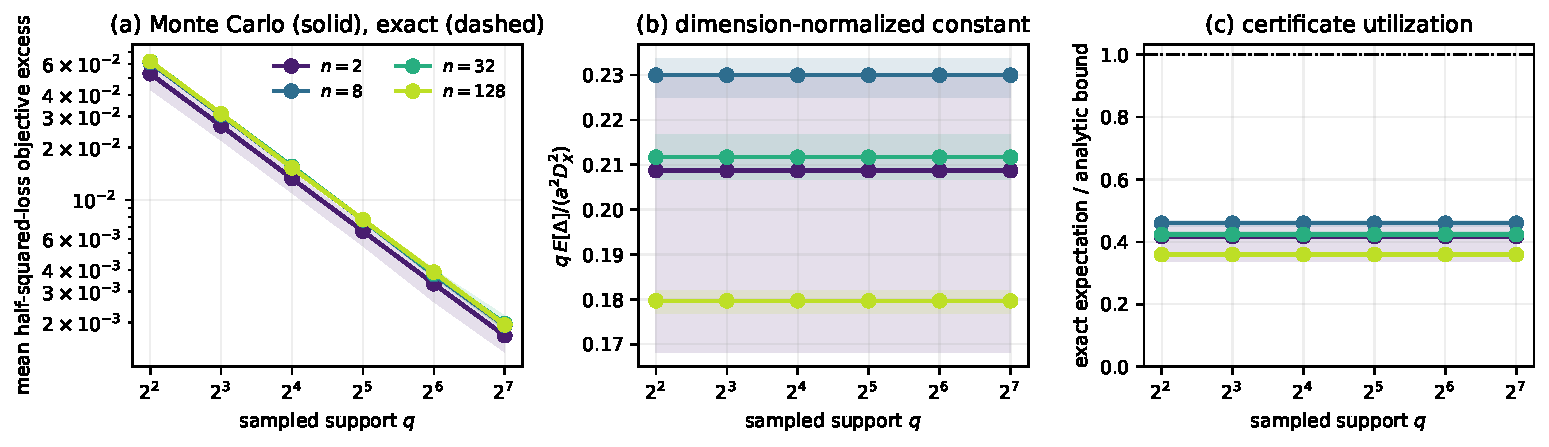
\includegraphics[width=\textwidth]{figures/Fig1.pdf}
\caption{Fixed-dictionary self-sparsification on dense width-256 endpoints.
Solid curves in (a) are Monte Carlo means and dashed curves are the exact
conditional expectations in \eqref{eq:empirical-exact-sampling}; bands are
the full ranges over eight endpoints. Panel (b) removes the theorem's
$q^{-1}$ scale and the data constant. Panel (c) divides the exact expectation
by the analytic smooth bound; the dash-dotted line is one.  This finite
computation checks the implementation and illustrates the mechanism; it is
not evidence for a barrier lower bound or a uniform population statement}
\label{fig:self-sparsification}
\end{figure}

Across all 192 endpoint--support settings, every one of the 2048 sampled
coefficient vectors has support at most $q$ and preserves the $\ell_1$ mass
to the recorded floating-point precision.  The largest exact-to-bound ratio
is $0.4672$.  After normalization, the complete range is
$q\E_I\Delta/(a^2D_X^2)\in[0.1683,0.2336]$ across input dimensions from two to
128.  The largest relative discrepancy between the Monte Carlo mean and the
closed-form expectation is $0.114$.  Thus the observed dimension changes the
finite covariance constant but does not introduce a different power of $q$.

\begin{table}[t]
\caption{Fixed-dictionary self-sparsification diagnostic. The slope is fitted only as an implementation check; the exact conditional expectation is algebraically proportional to $q^{-1}$. Ranges are over eight dense endpoints and all sampled supports}
\label{tab:self-sparsification}
\centering
\begin{tabular}{rrrr}
\toprule
$n$ & fitted slope & max. bound ratio & range of $q\mathbb E\Delta/(a^2D_X^2)$ \\
\midrule
2 & -1.000 & 0.461 & [0.168, 0.230] \\
8 & -1.000 & 0.467 & [0.225, 0.234] \\
32 & -1.000 & 0.434 & [0.207, 0.217] \\
128 & -1.000 & 0.364 & [0.177, 0.182] \\
\bottomrule
\end{tabular}
\end{table}


The same records also check the transfer in
Theorem~\ref{thm:balancing-retraction}.  The square-root lift
$\theta_i^{\rm raw}=\operatorname{sgn}(a_i)\sqrt{\abs{a_i}}$ and
$w_i^{\rm raw}=\sqrt{\abs{a_i}}u_i$ changes the stored predictions by at most
$4.45\times10^{-16}$ and the regularizer by at most
$1.74\times10^{-18}$.  These are invariant checks, not numerical evidence for
the global deformation-retraction claim.

\subsection{Complementary Complete-Path Stress Test}

We retain one complementary diagnostic from the earlier audit because
self-sparsification is only the endpoint-compression step: the theorem also
uses zero-output relocation, a common reference, and labeled coefficient
transfers.  On finite ridge-teacher distributions in dimensions
$n\in\{1,2,4\}$, ten independent pools contain eight projected-proximal-Adam
solutions at each width $m\in\{8,16,32,64,128\}$.  Three disjoint endpoint
pairs are selected per replicate and level.  The constructive path uses the
earlier deterministic cluster compression, followed by exactly the same
zero-buffer/reference part of the proof.  It is compared with direct
interpolation and a mesh-corrected Dynamic String Sampling (DSS) search.  This
test is therefore evidence that the complete path implementation is coherent,
not a second test of the dimension-free sampling rate.

Every nonconstant segment of the constructive path is coefficient
interpolation at fixed first-layer rows, so convexity makes the largest stored
node value an exact upper bound for that complete continuous path.  The DSS
and direct-interpolation values include the segmentwise mesh correction from
the globally Lipschitz Huber objective.  The selected levels are optimizer
proxies and the returned values are upper bounds for finitely many pairs; no
barrier lower bound or full-sublevel estimate is inferred.

\begin{figure}[t]
\centering
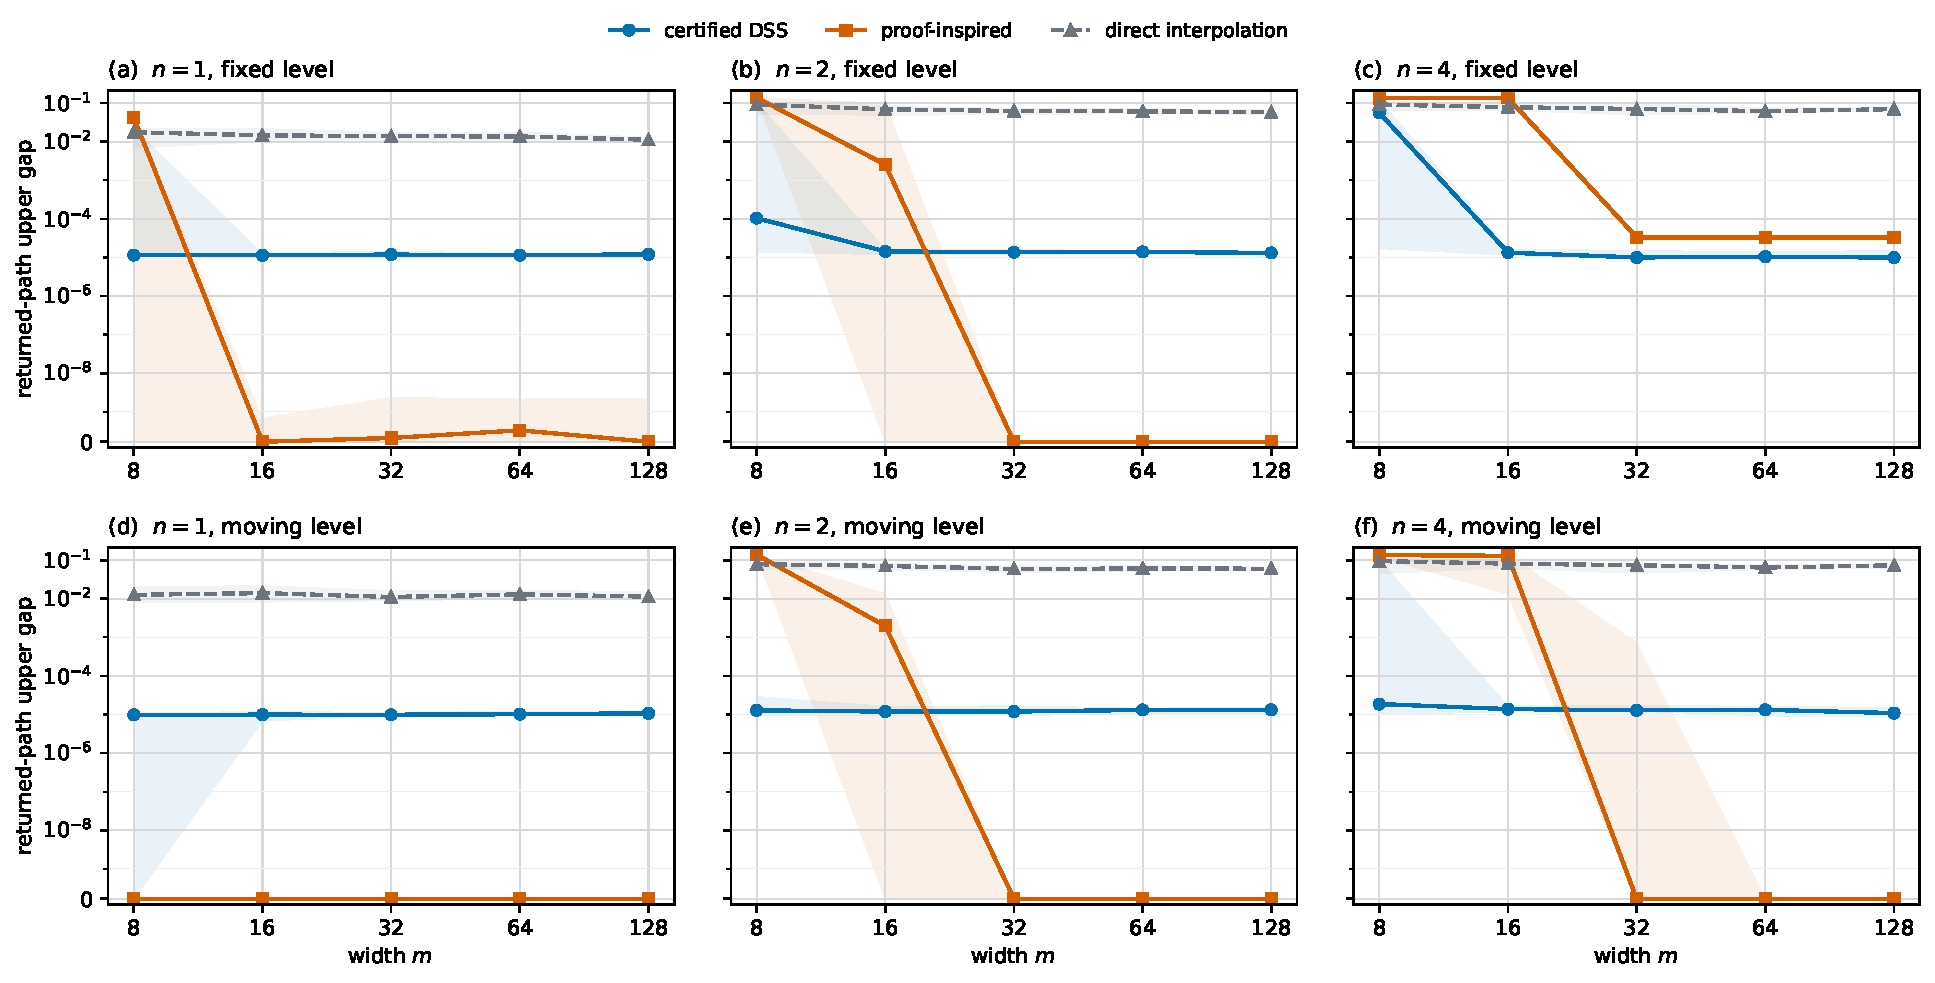
\includegraphics[width=\textwidth]{figures/Fig2.pdf}
\caption{Upper gaps of three complete returned paths. Columns are input
dimensions and rows separate a common fixed level from an optimizer-based
moving level. Each curve is the median of ten replicate-wise maxima over three
disjoint pairs; shading is the full replicate range. The sharp $m=8$ to
$m=16$ transition and the DSS tolerance floor should not be read as a fitted
asymptotic exponent}
\label{fig:path-diagnostics}
\end{figure}

For all 720 recorded Huber pairs with $m\ge16$, the smaller of the certified
DSS and constructive upper gaps is at most $1.6584\times10^{-5}$, or at most
$1.4391\times10^{-3}$ of the selected level.  Direct interpolation is much
higher: its median gap is $4.79\times10^{-2}$.  Table~\ref{tab:main-computation}
separates these finite path observations from the optimization proxy and the
legacy cluster-certificate check.

\begin{table}[t]
\caption{Frozen main-run summary. All path quantities are upper gaps for the recorded endpoint pairs, not estimates of the uniform sublevel barrier. The three path columns use only $m\ge16$; the compression ratio uses all widths. ``Best path'' means the smaller of the certified DSS and exact constructive upper gaps; $B$ is the analytic cluster-merge increment bound}
\label{tab:main-computation}
\centering
\scriptsize
\setlength{\tabcolsep}{3pt}
\begin{tabular}{@{}ccccccc@{}}
\toprule
$n$ & $\widehat e(8)$ & $\widehat e(128)$ & zero constructive & max best-path & median direct/DSS & max $\Delta_{\rm cmp}/B$ \\
 & & & gap (\%) & gap & ratio & \\
\midrule
1 & 0.117451 & 0.117451 & 90.8 & 2.338e-09 & 9.94e+02 & 0.089 \\
2 & 0.023544 & 0.023544 & 90.0 & 1.600e-05 & 4.60e+03 & 0.066 \\
4 & 0.010836 & 0.010721 & 35.8 & 1.658e-05 & 6.10e+03 & 0.045 \\
\bottomrule
\end{tabular}
\end{table}


\medskip
\noindent
Online Resource~1 contains supplementary reproducibility and proof-audit notes,
including frozen experimental parameters, implementation details,
path-certificate definitions, and provenance information.
